
协程是可以暂停执行并在稍后继续执行的函数,可以以与编写同步代码非常相似的方式编写异步代码。与使用\texttt{std::async}编写异步代码相比,这允许编写更清晰、更容易理解和维护的代码。不需要再写回调函数,也不需要用promise和future来处理\texttt{std::async}。

除此之外,还可以为提供更好的性能。基于\texttt{std::async}的代码通常在切换线程和等待方面有更多的开销。与调用函数的开销相比,协程可以非常快捷地恢复和挂起,这意味着可以产生更好的延迟和吞吐量。此外,其设计目标是具有高度的可扩展性,甚至可以扩展到数十亿个并发协程。

\begin{center}
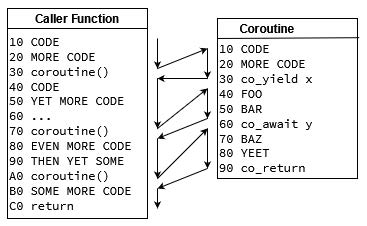
\includegraphics[width=0.6\textwidth]{content/3/chapter11/images/1.jpg}\\
图11.1 -调用和执行协程与使用常规函数不同,因为它们可以挂起和恢复
\end{center}

C++协程无堆栈,它们的状态不存储在调用线程的堆栈上。这给了它们一个有趣的属性:几个不同的线程可以执行一个协程。换句话说,尽管协程函数体看起来是按顺序执行的,但某些部分可以在不同的线程中执行。这使得将函数的一部分留给专用线程来执行成为可能。例如,I/O操作可以在专用的I/O线程中完成。

要检查函数是否为C++协程,需要在函数体中查找以下关键字:

\begin{itemize}
\item 
\texttt{co\_await},暂停协程。

\item 
\texttt{co\_yield}用于向调用方返回值,并暂停协程。

\item 
类似于Python在生成器中使用的\texttt{yield}关键字,允许惰性生成值。

\item 
co\_return,返回一个值并完成协程的执行,与\texttt{return}关键字等价。
\end{itemize}

只要函数体中有其中一个关键字,函数就会自动变成协程。虽然这是一个实现细节,但还有一个提示:协程返回类型必须满足某些要求(后面再说)。

协程是C++世界中的一等公民,可以获取它们的地址,用作函数参数,从函数返回它们,并将它们存储在对象中。

在C++中,可以在C++20之前编写协程。这要感谢Boost等库。Coroutine2,也就是彭博的Quantum。后者用来实现CoroKafka——使用协程高效处理Kafka流的库。随着标准C++协程的出现,新的库开始出现。现在,将向展示其中一个。

\subsubsubsection{11.5.1\hspace{0.2cm}与cppcoro的区别}

从头编写基于协程的代码很困难。C++20只提供了编写协程的基本实用程序,所以在编写自己的协程时需要一组原语。Lewis Baker创建的cppcoro库是C++中最常用的协程框架之一。本节中,将展示这个库,并演示如何在编写基于协程的代码时使用它。

先来概述一下库提供的协程类型:

\begin{itemize}
\item 
\texttt{task<>}: 为了调度工作稍后执行——当\texttt{co\_await}开始执行。

\item 
\texttt{shared\_task<>}: 多个协程可以等待一个任务。可以复制,以便多个协程引用相同的结果。本身没有提供任何线程安全性。

\item 
\texttt{generator}: 缓慢而同步地产生一个T序列。它实际上是\texttt{std::range},它有一个返回迭代器的\texttt{begin()}和一个返回哨兵的\texttt{end()}。

\item 
\texttt{recursive\_generator}: 类似于\texttt{generator<T>},但可以生成\texttt{T}或\texttt{recursive\_generator<T>}。这里会有一些额外的开销。

\item 
\texttt{async\_generator}: 类似于\texttt{generator<T>},但是可以异步生成值。这意味着,与生成器相反,异步

\item 
生成器可以在它们的函数体内使用\texttt{co\_await}。
\end{itemize}

应该使用这些类型作为协程的返回类型。通常,在生成器中(协程返回前面的生成器类型),可以使用\texttt{co\_yield}的返回值(类似于Python生成器)。然而,在任务中,通常需要使用\texttt{co\_await}来安排工作。

与前面的协程类型相比,这个库实际上提供了更多的编程抽象。还提供以下类型:

\begin{itemize}
\item 
\texttt{co\_await}的可等待类型,比如协程事件和同步原语:互斥锁、锁存、栅栏等。

\item 
可取消,可以取消协程的执行。

\item 
调度器——可以调度工作的对象,例如\texttt{static\_thread\_pool},或在特定线程上调度工作。

\item 
I/O和网络工具,允许读写文件和IP套接字。

\item 
元函数和概念,比如\texttt{awaitable\_traits}、\texttt{awaitable}和\texttt{Awaiter}。
\end{itemize}

除了前面的实用程序之外,cppcoro还提供了一些函数——用于使用其他类和指导执行的程序,例如:

\begin{itemize}
\item 
\texttt{sync\_wait}: 阻塞式,直到传递的可等待对象完成工作。

\item
\texttt{when\_all},\texttt{when\_all\_ready}: 返回一个可等待对象,该对象在传递的所有可等待对象完成时完成。这两者之间的区别在于处理子可等待对象的失败。即使在失败的情况下,\texttt{when\_all\_ready}将完成,调用者可以检查每个结果,而\texttt{when\_all}将重新抛出一个异常,如果任何子可等待对象抛出一个异常(虽然不知道是哪个),其还会取消所有未完成的任务。

\item
\texttt{fmap}: 与函数式编程类似,将函数应用于可等待对象。可以将其视为将一种类型的任务转换为另一种类型的任务。例如,可以通过调用\texttt{fmap(serialize, my\_coroutine())}来序列化协程返回的类型。

\item
\texttt{resume\_on}: 指示协程在完成某些工作后,使用哪个调度器继续执行。这能够在特定的执行上下文中执行特定的工作,例如在专用的I/O线程上运行与I/O相关的任务。注意,这意味着一个C++函数(协程)可以在单独的线程上执行它的各个部分。可以使用类似于\texttt{std::ranges}的计算“通道”。

\item
\texttt{schedule\_on}: 指示协程使用哪个调度器来启动某些工作。通常用法\texttt{auto foo = co\_await schedule\_on(scheduler, do\_work());}。
\end{itemize}

在开始使用这些实用程序之前,再了解一下可等待程序。

\subsubsubsection{11.5.2\hspace{0.2cm}剖析可等待程序和协程}

除了cppcoro之外,标准库还提供了两个可等待对象:\texttt{suspend\_never}和\texttt{suspend\_always}。通过了解它们,可以看到如何在需要时实现自己的可等待对象:

\begin{lstlisting}[style=styleCXX]
struct suspend_never {
	constexpr bool await_ready() const noexcept { return true; }
	constexpr void await_suspend(coroutine_handle<>) const noexcept {}
	constexpr void await_resume() const noexcept {}
};

struct suspend_always {
	constexpr bool await_ready() const noexcept { return false; }
	constexpr void await_suspend(coroutine_handle<>) const noexcept {}
	constexpr void await_resume() const noexcept {}
};
\end{lstlisting}

当输入\texttt{co\_await}时,告诉编译器首先调用等待者的\texttt{await\_ready()}。如果返回true表示已经准备好了,\texttt{await\_resume()}将调用。\texttt{await\_resume()}的返回类型应该是等待者实际生成的类型。如果没有准备好,程序将执行\texttt{await\_suspend()}。完成后,有三种情况:

\begin{itemize}
\item 
\texttt{await\_suspend}返回\texttt{void}:执行之后总是挂起。

\item 
\texttt{await\_suspend}返回\texttt{bool}:执行是否挂起取决于返回值。

\item 
\texttt{await\_suspend}返回\texttt{std::coroutine\_handle<PromiseType>}:另一个协程将恢复运行。
\end{itemize}

协程的背后还有更多的东西。即使协程不使用\texttt{return}关键字,编译器也会在后台生成代码,使它们能够编译和工作。当使用诸如\texttt{co\_yield}这样的关键字时,将把它们重写为对协助类型的适当成员函数的调用。例如,对\texttt{co\_yield x}的调用等价于\texttt{co\_await promise.yield\_value(x)}。如果想进一步了解协程更多信息,并编写自己的协程类型,请参阅扩展阅读部分的《第一个协程》。

好了,让我们用这些知识来写自己的协程吧。我们将创建一个简单的应用程序来模拟有意义的工作,这里现来使用一个线程池来用一些数字填充向量。

CMake目标如下:

\begin{lstlisting}[style=styleCMake]
add_executable(coroutines_1 coroutines/main_1.cpp)
target_link_libraries(coroutines_1 PRIVATE cppcoro fmt::fmt
Threads::Threads)
target_compile_features(coroutines_1 PRIVATE cxx_std_20)
\end{lstlisting}

将链接到cppcoro库。在例子中,使用的是Andreas Buhr的cppcoro分支,因为它是Lewis Baker仓库的一个维护良好的分支,并且支持CMake。

还将链接到用于文本格式化的优秀\{fmt\}库。如果标准库提供了C++20的字符串格式,可以使用标准库的格式化方法。

最后,需要一个线程库——希望在池中使用多个线程。

以一些常量和一个main函数开始实现:

\begin{lstlisting}[style=styleCXX]
inline constexpr auto WORK_ITEMS = 5;

int main() {
	auto thread_pool = cppcoro::static_thread_pool{3};
\end{lstlisting}

希望使用三个池中的线程生成五个元素,cppcoro的线程池以一种简单的方法对工作进行安排。默认情况下,创建的线程数量与机器的硬件线程数量相同。接下来,需要具体说明相应的工作:

\begin{lstlisting}[style=styleCXX]
fmt::print("Thread {}: preparing work\n", std::this_thread::get_id());
auto work = do_routine_work(thread_pool);

fmt::print("Thread {}: starting work\n", std::this_thread::get_id());
const auto ints = cppcoro::sync_wait(work);
\end{lstlisting}

在代码中散布日志消息,这样就可以更好地看到在哪个线程中发生了什么。可以通过调用名为\texttt{do\_routine\_work}的协程来创建工作。返回协程,使用\texttt{sync\_wait}阻塞函数运行协程,协程只有在实际待时才会执行。这样,实际工作的将在这个函数调用中开始。

当运行有了结果,就可以把结果记录下来:

\begin{lstlisting}[style=styleCXX]
fmt::print("Thread {}: work done. Produced ints are: ",
			std::this_thread::get_id());
for (auto i : ints) {
	fmt::print("{}, ", i);
}
fmt::print("\n");
\end{lstlisting}

定义我们的\texttt{do\_routine\_work}协程:

\begin{lstlisting}[style=styleCXX]
cppcoro::task<std::vector<int>>
do_routine_work(cppcoro::static_thread_pool &thread_pool) {
	auto mutex = cppcoro::async_mutex{};
	auto ints = std::vector<int>{};
	ints.reserve(WORK_ITEMS);
\end{lstlisting}

它返回一个任务,该任务生成一些整数。因为使用线程池,所以让使用cppcoro的\texttt{async\_mutex}来同步线程。现在来使用池:

\begin{lstlisting}[style=styleCXX]
fmt::print("Thread {}: passing execution to the pool\n",
			std::this_thread::get_id());
co_await thread_pool.schedule();
\end{lstlisting}

\texttt{schedule()}调用没有传入可调用对象来执行,在协程的情况下,实际上当前线程暂停协程。并开始执行它的调用程序。现在将等待协程完成(在\texttt{sync\_wait}调用的地方)。

与此同时,池中的一个线程将恢复协程——继续执行它的任务。以下是为此所做的准备:

\begin{lstlisting}[style=styleCXX]
fmt::print("Thread {}: running first pooled job\n",
			std::this_thread::get_id());
			
std::vector<cppcoro::task<>> tasks;
for (int i = 0; i < WORK_ITEMS; ++i) {
	tasks.emplace_back(
		cppcoro::schedule_on(thread_pool, fill_number(i, ints, mutex)));
}
co_await cppcoro::when_all_ready(std::move(tasks));
co_return ints;
\end{lstlisting}

我们创建一个要执行的任务集,每个任务在互斥锁下填充一个整数。\texttt{schedule\_on}调用池中的另一个线程运行填充协程。最后,等待所有的结果。此时,任务开始执行。最后,由于协程是一个任务,这里使用\texttt{co\_return}。

\begin{tcolorbox}[colback=blue!5!white,colframe=blue!75!black, title=Note]
\hspace*{0.7cm}不要忘记\texttt{co\_return}生成的值。如果移除\texttt{co\_return int;},将简单地返回一个默认构造的数组。程序将运行,打印空数组,并以代码0退出。
\end{tcolorbox}

最后一步是实现产生数字的协程:

\begin{lstlisting}[style=styleCXX]
cppcoro::task<> fill_number(int i, std::vector<int> &ints,
cppcoro::async_mutex &mutex) {
	fmt::print("Thread {}: producing {}\n", std::this_thread::get_id(), i);
	std::this_thread::sleep_for(
		std::chrono::milliseconds((WORK_ITEMS - i) * 200));
\end{lstlisting}

这个任务不返回任何值。相反,会把它加到数组上。繁重工作实际上是通过休眠几毫秒来完成的。睡醒后,协作程序将继续进行更有成效的工作:

\begin{lstlisting}[style=styleCXX]
{
	auto lock = co_await mutex.scoped_lock_async();
	ints.emplace_back(i);
}
\end{lstlisting}

它将锁定互斥对象。其实,只是等待而已。当互斥锁锁定时,会给\texttt{vector}添加一个数字——与调用时相同的数字。

\begin{tcolorbox}[colback=blue!5!white,colframe=blue!75!black, title=Note]
\hspace*{0.7cm}还记得\texttt{co\_await}么?如果记不清了,可以不使用可等待对象(可能因为不使用每个可等待对象也是可以的),那么就会跳过一些必要的计算。在例子中,这可能代表着不锁定互斥对象。
\end{tcolorbox}

现在来完成协程的实现:

\begin{lstlisting}[style=styleCXX]
 fmt::print("Thread {}: produced {}\n", std::this_thread::get_id(), i);
co_return;
\end{lstlisting}

一个简单的状态打印和一个\texttt{co\_return}来标记协程完成。返回时,协程框架就可以销毁了,释放其占用的内存。

这是所有了!现在运行代码,看看会发生什么:

\begin{tcblisting}{commandshell={}}
Thread 140471890347840: preparing work
Thread 140471890347840: starting work
Thread 140471890347840: passing execution to the pool
Thread 140471890282240: running first pooled job
Thread 140471890282240: producing 4
Thread 140471881828096: producing 1
Thread 140471873373952: producing 0
Thread 140471890282240: produced 4
Thread 140471890282240: producing 3
Thread 140471890282240: produced 3
Thread 140471890282240: producing 2
Thread 140471881828096: produced 1
Thread 140471873373952: produced 0
Thread 140471890282240: produced 2
Thread 140471890347840: work done. Produced ints are: 4, 3, 1, 0, 2,
\end{tcblisting}

主线程用于启动池上的工作,然后等待结果。然后,池中的三个线程产生数字。最后安排的任务实际上是第一个运行的任务,产生数字4。这是因为它一直在执行\texttt{do\_routine\_work}:首先,调度池中的其他任务,然后在调用\texttt{when\_all\_ready}时开始执行第一个任务。稍后,执行继续进行,第一个空闲线程接受池上调度的下一个任务,直到整个数组填满。最后,执行返回到主线程。

这个例子到此结束。通过它,我们就结束了本章的最后一部分。现在来回顾一下本章了解到的内容。


